\documentclass[aspectratio=43]{beamer}
\usepackage[utf8]{inputenc}
\usepackage{macros}


\title{Quantum Algorithms}
\date{November, 2018}
\author[Ramalho]{Miguel Sozinho Ramalho}
% \institution[FEUP]{Faculty of Engineering of the University of Porto}

%%%%%%%%%%%%%%%%%%%%%%%% THEME
\usetheme{material}
\useLightTheme
\usePrimaryIndigo
\useAccentRed


\begin{document}

\begin{frame}
	\titlepage
\end{frame}


\begin{frame}{Table of contents}
	\begin{card}
		\tableofcontents
	\end{card}
\end{frame}


\section{Introduction}
\begin{frame}{Introduction}
    \begin{card}
        Time has come for us to effectively show how a quantum computer might beat a classical one. For this, we will explore the \ds algorithm (and its general case \djs). It does not solve a particularly interesting problem in classical computer science, but it does highlight the \textit{quantum power}, so to speak. Some previous notions on \textbf{\q Oracles} and \textbf{Reversible Computation} are also presented.
    \end{card}
\pagenumber
\end{frame}

\section{\q Oracles}
\begin{frame}{\q Oracles}
\begin{card}
    No, we are not about to delve into  \href{https://en.wikipedia.org/wiki/The_Oracle_(The_Matrix)}{Matrix's Oracle}.\\
    \q Oracles are actually a useful abstraction for writing quantum algorithms. An Oracle hides a function that takes a number of qubits as input, performs a transformation, and produces the same number of qubits as output. It can be seen as black box:
    \begin{center}
        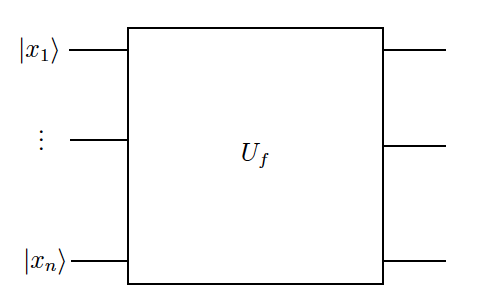
\includegraphics[width=0.5\textwidth]{oracle}
    \end{center}
\end{card}
\pagenumber
\end{frame}

\begin{frame}{\q Oracles}
\begin{card}
    Some of the reasons for using oracles are:
    \begin{itemize}
        \item Conceptual simplification of circuits
        \item Allows for the comparison between classical and quantum algorithms
        \item Eases the visual interpretation of quantum circuits
    \end{itemize}
\end{card}
\begin{card}
    As we will see, this concept is quite used in the specification of new quantum algorithms, as it allows us to abstract from the unnecessary, following the lines of the computer science  \href{https://en.wikipedia.org/wiki/Abstraction_principle_(computer_programming)}{Abstraction Principle}. 
\end{card}
\pagenumber
\end{frame}

\section{\q Reversible Computation}
\begin{frame}{\q Reversible Computation}
\begin{card}
    We want quantum computations to be \textbf{reversible}, and that is an intended consequence of the \textbf{unitary} nature of quantum gates. However, we must also be able to extrapolate this notion of \textbf{reversibility to oracles}, so that we can be sure (through a sort of implicit induction) that we do not lose the property of reversibility regardless of the complexity of our circuit.
\end{card}
\pagenumber
\end{frame}

\begin{frame}{\q Reversible Computation}
    Consider a classical circuit for computing a Boolean operator:
    \begin{center}
        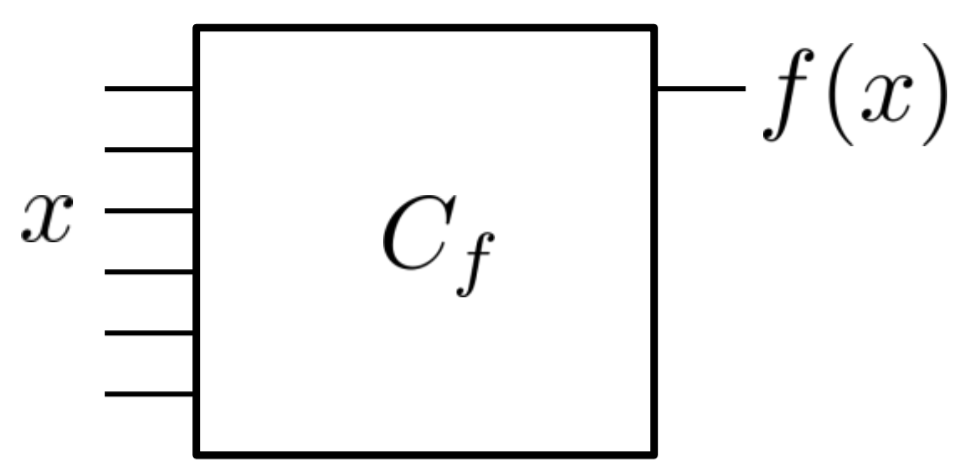
\includegraphics[width=0.35\textwidth]{classic_operator}
    \end{center}
    \small{If we were to do this in quantum circuits, we would lose all the information about x and, therefore, destroy any chance of reversibility. What we really want is a way we can apply the reverse gate of $U_f$, $U_f^\dag$:}
    \begin{center}
        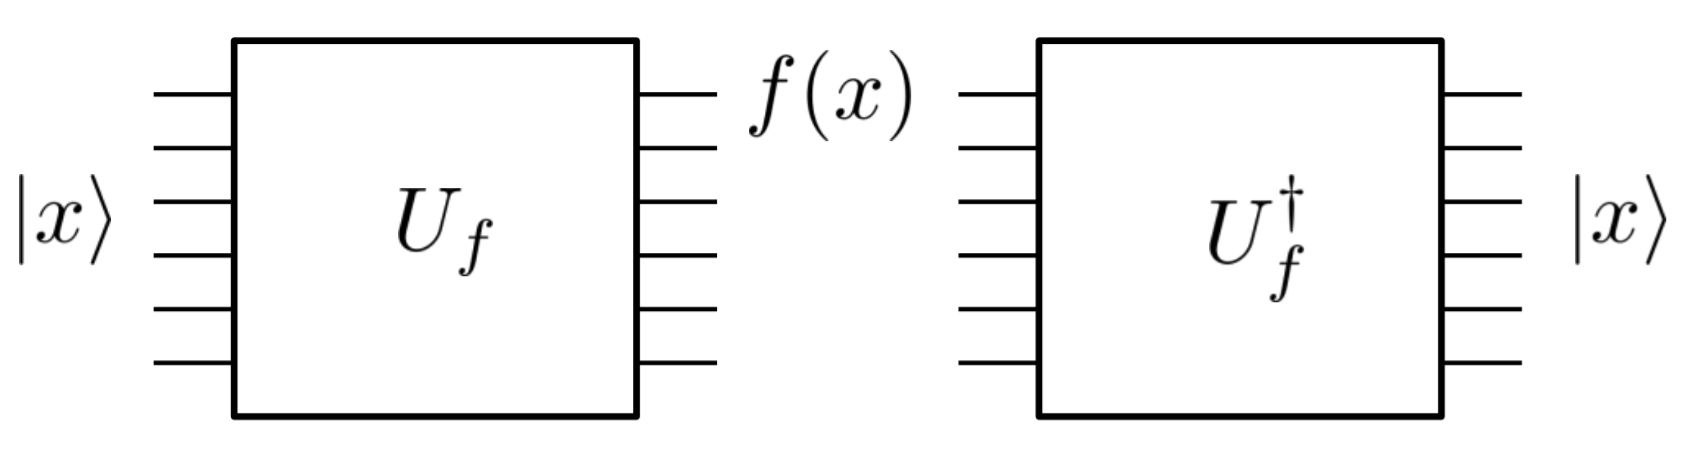
\includegraphics[width=0.65\textwidth]{quantum_operator}
    \end{center}
\pagenumber
\end{frame}

\begin{frame}{\q Reversible Computation}
    Achieving this is easier than it looks. We already have the tools!\\
    We are already able to compute any function and then reverse it back to the original state, as we only use unitary operators. But doing this means going back to the start. However, if we use some \textit{helper qubits}, we may be on to something...
    \begin{center}
        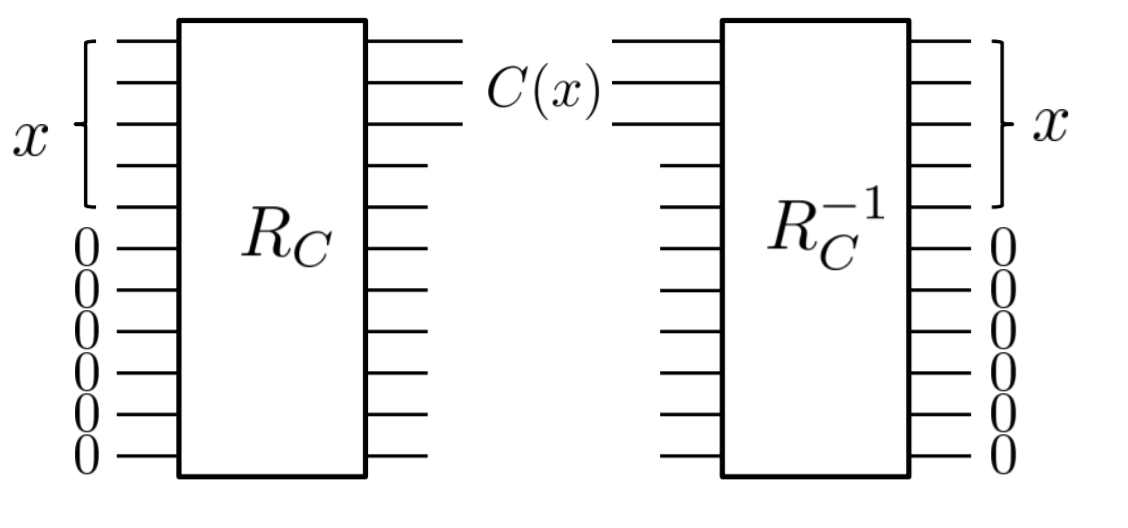
\includegraphics[width=0.7\textwidth]{reversible_01}
    \end{center}
\pagenumber
\end{frame}

\begin{frame}{\q Reversible Computation}
    Indeed! Have you noticed the CNOT gate's equivalent in logical gates is the exclusive OR (XOR), and it can be used to copy the result of $C(x)$ onto the $y$ qubits, if each of those qubits in $y=\kz$ (0 XOR A = A).
    \begin{center}
        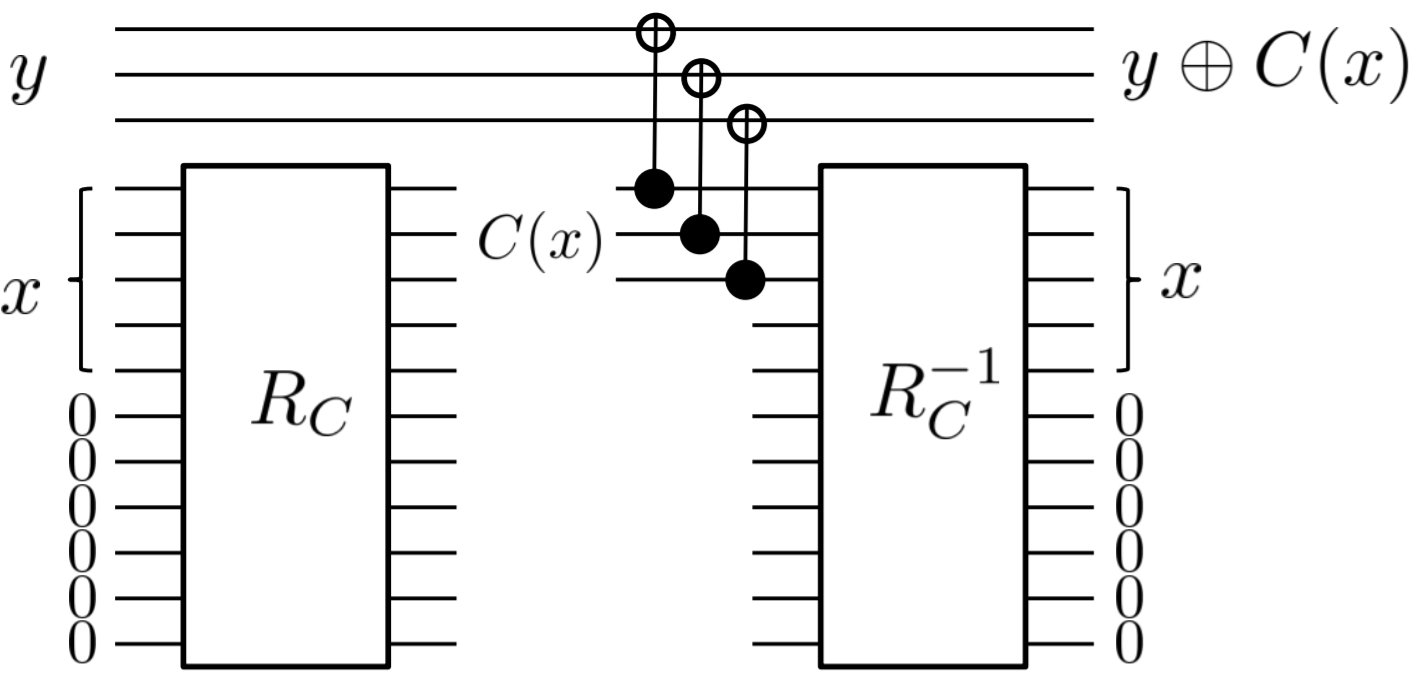
\includegraphics[width=0.7\textwidth]{reversible_02}
    \end{center}
\pagenumber
\end{frame}


\begin{frame}{\q Reversible Computation}
    This means we can obtain our inductive reversibility notion if we apply the operations we want on our input qubits, save it using as many CNOT gates as the number of qubits in the result, and reverting the qubits we obtained by applying the inverse operations to go back to the original input. The difference being we also have the result!
    \begin{center}
        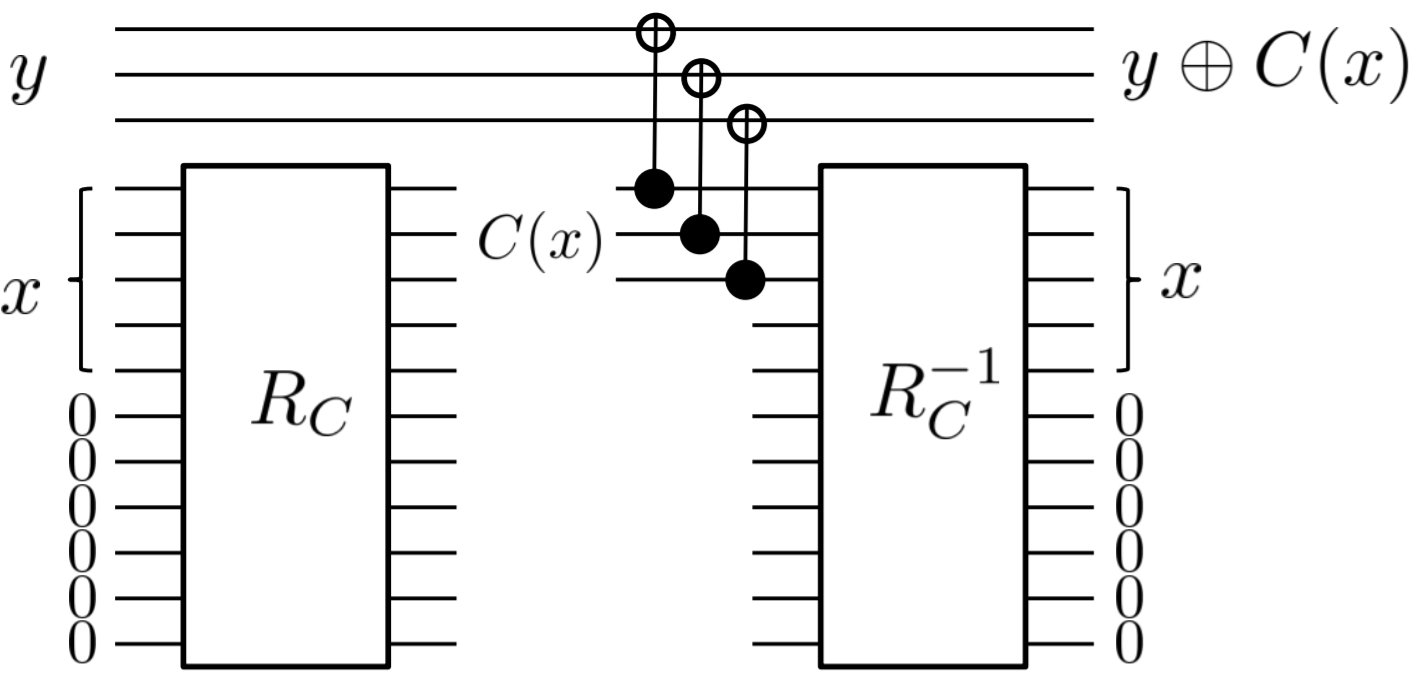
\includegraphics[width=0.7\textwidth]{reversible_02}
    \end{center}
\pagenumber
\end{frame}

\begin{frame}{\q Reversible Computation}
    In the end, even though we need some extra zeroed qubits, we can abstract our circuit onto a reversible mapping, since we never loose, only gain, information! \textit{et voila}:
    \begin{center}
        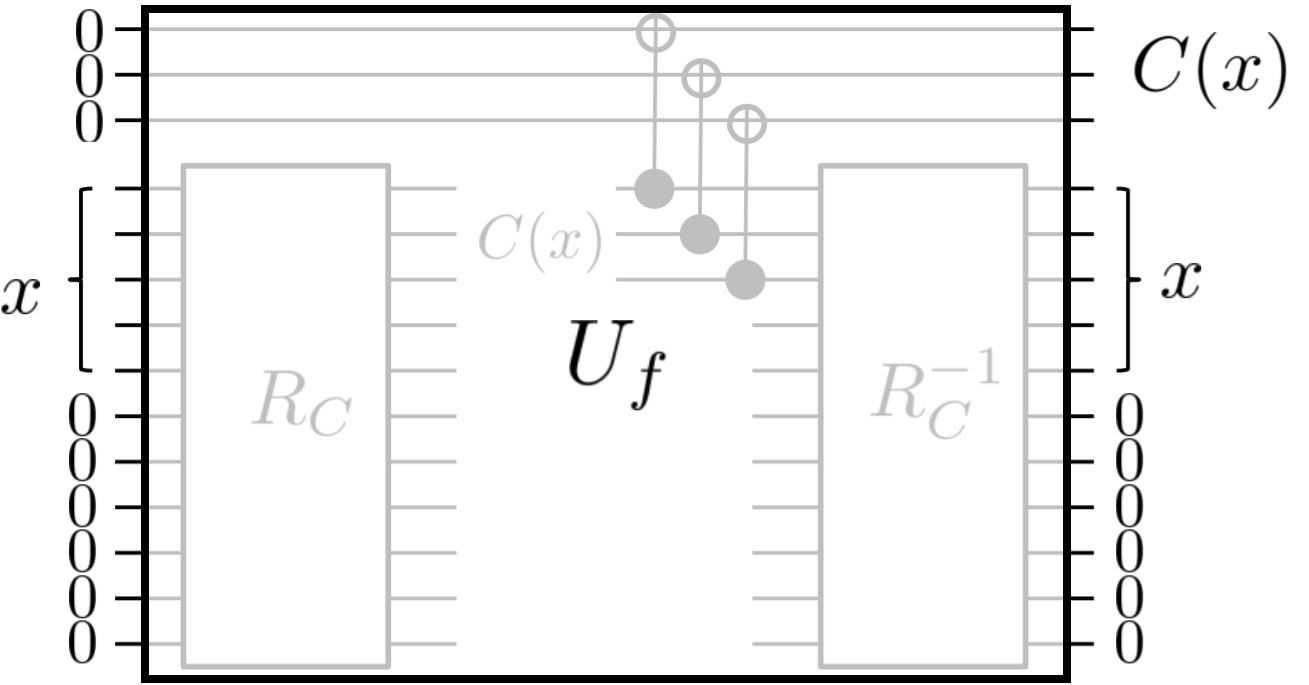
\includegraphics[width=0.7\textwidth]{reversible_04}
    \end{center}
\pagenumber
\end{frame}


\section{Deutsch-Jozsa Problem Formulation}
\begin{frame}{\djs Problem Formulation}
\begin{card}
    Consider a function $f: \{0,1\}^n \rightarrow \{0,1\}$ that maps an array of $n$  bits into either 0 or 1. We do not know the logic behind it. We know that it is either constant or balanced:
    \begin{description}
        \item[Constant:] its output is always 0 or always 1
        \item[Balanced:] outputs 0 for half the input value and 1 for the other half
    \end{description}
\end{card}
\pagenumber
\end{frame}

\section{Deutsch's Problem Formulation}
\begin{frame}{\ds Problem Formulation}
\begin{card}
    For the case that $n=1$ we have $f: \{0,1\} \rightarrow \{0,1\}$ that maps a single bit into either 0 or 1. If we are given a black box, an \textbf{oracle}, that takes as input this two bits and outputs the unknown value:
    \begin{center}
        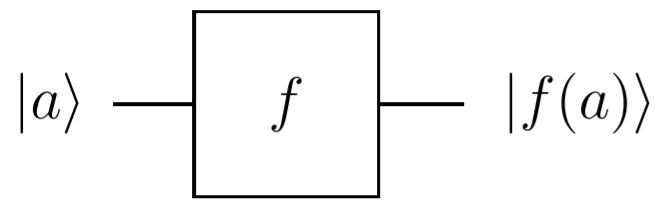
\includegraphics[width=0.5\textwidth]{classic_black_box}
    \end{center}
\end{card}
\begin{cardTiny}
    To answer this question classically, we would always need two function invocations. We could do $f(0)$ and $f(1)$ and see if it is either constant or balanced. 
\end{cardTiny}
\pagenumber
\end{frame}

\begin{frame}{Classical Algorithm}
\begin{card}
    \begin{center}
        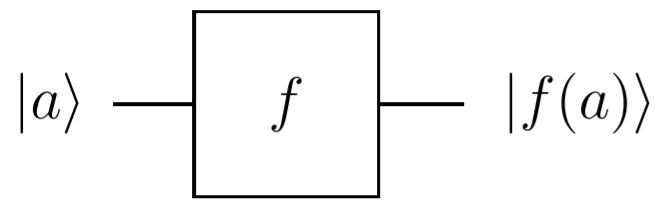
\includegraphics[width=0.5\textwidth]{classic_black_box}
    \end{center}
\end{card}
\begin{cardTiny}
    An alternative would be to check what the value of $f(0)$ XOR $f(1)$ would produce:
    \begin{equation*}
        \left\{\begin{matrix}
            f(0)\text{ XOR } f(1) = 0 \rightarrow constant\\ 
            f(0)\text{ XOR } f(1) = 1 \rightarrow balanced\\ 
        \end{matrix}\right.
    \end{equation*}
    Yet, this would still require two invocations of the black box.
\end{cardTiny}
\pagenumber
\end{frame}


\begin{frame}{\q Algorithm}
\begin{card}
    Before transforming it into a quantum problem, we need our black box to be an oracle which allows for reversible computation, like so:
    \begin{center}
        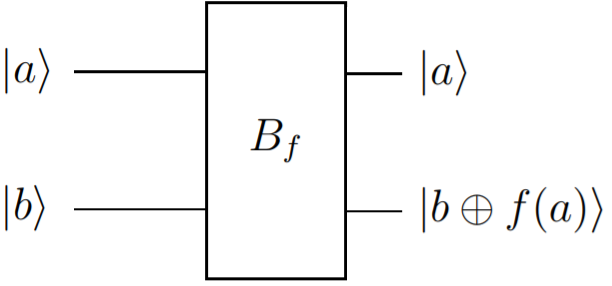
\includegraphics[width=0.5\textwidth]{quantum_black_box}
    \end{center}
\end{card}
\pagenumber
\end{frame}


\begin{frame}{\ds Algorithm}
Let us imagine the following procedure:\\
\begin{enumerate}
    \item We begin with two qubits, q0 in state $\kz$ and q1 in state $\ko$ ($\ket{01}$).
    \item We apply a Hadamard to each qubit, the result is $\frac{1}{2}(\ket{00} - \ket{01} + \ket{10} - \ket{11})$
    \item We now call our oracle, which maps $\ket{a b}$ or $\ket{a}\ket{b}$ (easier to interpret) into $\ket{a}\ket{b\oplus f(a)}$ the result is:
\end{enumerate}
\begin{equation}
     \frac{1}{2}(\kz\ket{0\oplus f(0)} - \kz\ket{1\oplus f(0)} + \ko\ket{0\oplus f(1)} - \ko\ket{1\oplus f(1)})
\end{equation}
\pagenumber
\end{frame}

\begin{frame}{\ds Algorithm}
Simplifying:
\begin{equation*}
    \frac{1}{2}(
        \kz [\ket{0\oplus f(0)} - \ket{1\oplus f(0)}]
        +  
        \ko [(\ket{0\oplus f(1)} - \ket{1\oplus f(1)}]
    )
\end{equation*}
We can now use the following equivalence:
\begin{equation*}
    \ket{0 \oplus a} - \ket{1 \oplus a} =  (-1)^a(\kz - \ko)
\end{equation*}
To replace above and get:
\begin{equation*}
    \frac{1}{2}(
        \kz [(-1)^{f(0)}(\kz - \ko)]
        +  
        \ko [(-1)^{f(1)}(\kz - \ko)]
    )
\end{equation*}
\pagenumber
\end{frame}


\begin{frame}{\ds Algorithm}
Separating back into the 2 qubit shape:
\begin{equation*}
    [\osqrt (-1)^{f\kz} \kz + \osqrt (-1)^{f(\kz}\kz][\osqrt \kz - \osqrt \ko]
\end{equation*}
Our second qubit : $(\osqrt \kz - \osqrt \ko)$ can be ignored, and what remains is our first qubit: $(\osqrt (-1)^{f\kz} \kz + \osqrt (-1)^{f(\kz}\kz)$ which contains both $f(0)$ and $f(1)$! both images of $f$ with a single pass over the oracle. This can further be simplified as:
\begin{equation*}
    (-1)^{f(0)}(\osqrt \kz + \osqrt (-1)^{f(0) \oplus f(1)} \ko)
\end{equation*}
\pagenumber
\end{frame}

\begin{frame}{\ds Algorithm}
Lastly, we apply a Hadamard gate on our qubit (go ahead and do this on paper) and we arrive at:
\begin{equation*}
    (-1)^{f(0)} \ket{f(0) \oplus f(1)}
\end{equation*}
\begin{cardTiny}
    What is the meaning of this? See for yourself!
    \begin{itemize}
        \item if f is constant ($00$ or $11$) $\rightarrow$ output is $0$ (xor is 0)
        \item if f is balanced ($01$ or $10$) $\rightarrow$ output is $\pm 1$ (xor is 1)
    \end{itemize}
    Which, in fact, means that we can do a\textbf{ single pass} over the oracle gate discover whether it is constant or balanced, an impossible feat in classical computing. 
\end{cardTiny}
\pagenumber
\end{frame}


\begin{frame}{\ds Algorithm}
All in all, what we did was follow the following circuit:
\begin{center}
    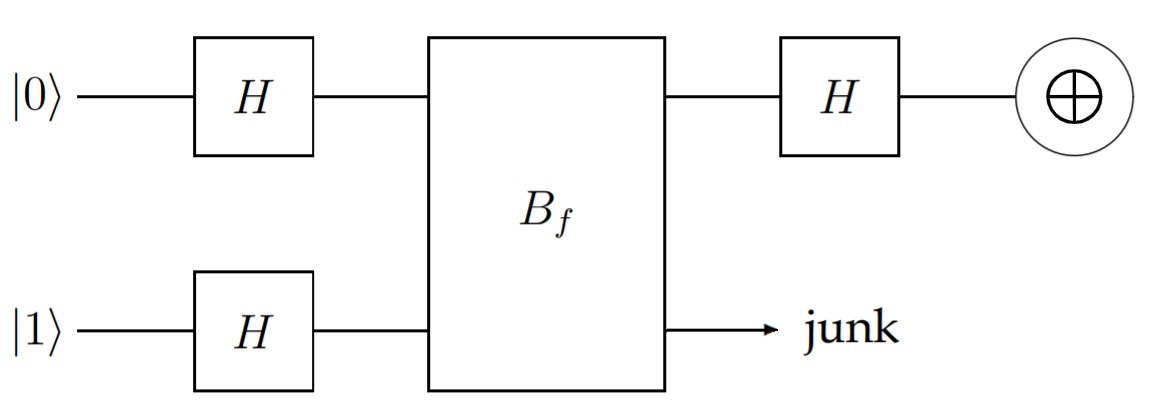
\includegraphics[width=0.8\textwidth]{deutsch_algorithm}
\end{center}
\begin{cardTiny}
    As you can see it is one of the simplest quantum circuits we could have designed but, nonetheless, it gave us some hard time understanding how and why it worked. Do not fear, for quantum algorithms are usually hard at the beginning as they demand a new way of tackling problems!
\end{cardTiny}
\pagenumber
\end{frame}

\section{Deutsch-Jozsa Algorithm}
\begin{frame}{\djs Algorithm}
\begin{card}
    If we go back to our function $f: \{0,1\}^n \rightarrow \{0,1\}$ it should be known that the solution to the $n=1$ instance is generalizes to answer the same question on an n-dimensional array with... can you guess how many passes over the black box..? \small{(Do note that a classical algorithm would need $2^{n-1}+1$ passes)}
    \begin{center}
        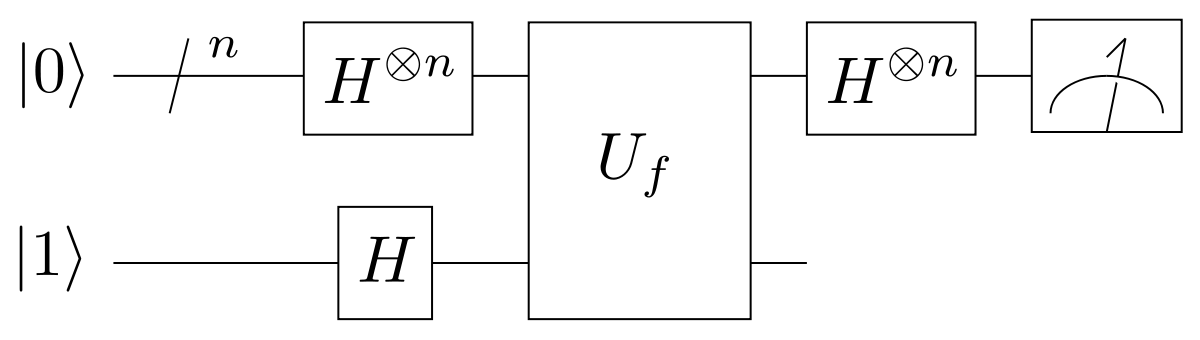
\includegraphics[width=0.8\textwidth]{deutsch_jozsa_algorithm}
    \end{center}
\end{card}
\pagenumber
\end{frame}

\begin{frame}{\djs Algorithm}
\begin{cardTiny}
    \begin{center}
        \Large{ONE!}
    \end{center}
\end{cardTiny}
\begin{card}
    Just one pass. By using n qubits initialized to 0 and 1 to 1, by performing the same operations, but on more qubits, again:
    \begin{center}
        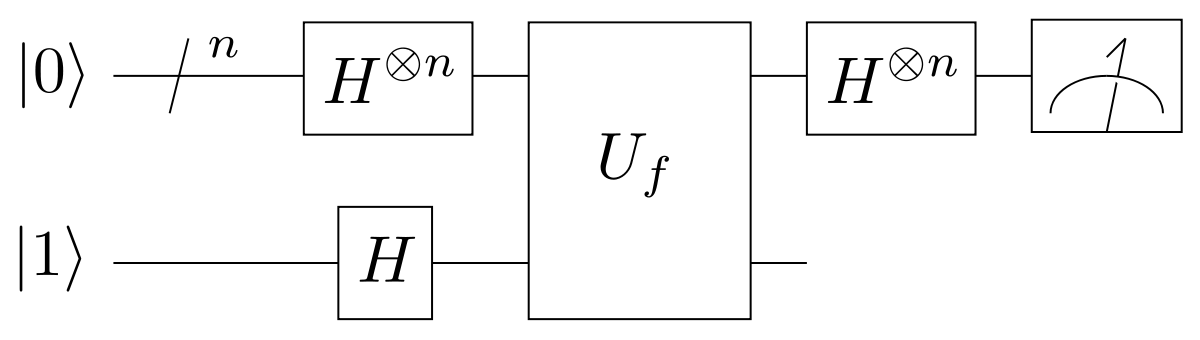
\includegraphics[width=0.8\textwidth]{deutsch_jozsa_algorithm}
    \end{center}
\end{card}
\pagenumber
\end{frame}


\section{Implementation Tips}
%https://github.com/Qiskit/ibmqx-user-guides/blob/master/rst/full-user-guide/004-Quantum_Algorithms/080-Deutsch-Jozsa_Algorithm.rst
\begin{frame}{Hands-on}
\begin{card}
    Although \qk does not allow for oracles, as it would require quite a challenging approach (remember it should be able to interact with real hardware), we can simply choose a couple of operations instead of a black box and implement our \ds algorithm around them, and that is precisely what you will get to do on this week's exercises!
\end{card}
\pagenumber
\end{frame}


\section{Where to learn more?}
\begin{frame}{Where to learn more?}
\begin{card}
    \begin{itemize}
    \item \href{https://www.youtube.com/watch?v=mGqyzZ-fnnY}{\djs on Youtube}
    \item \href{https://www.youtube.com/watch?v=-f_VTELFXxU}{\ds on Youtube}
    \item \href{http://rspa.royalsocietypublishing.org/content/439/1907/553}{The original \djs paper}
    \end{itemize}
\end{card}
\end{frame}
\end{document}
